% Options for packages loaded elsewhere
\PassOptionsToPackage{unicode}{hyperref}
\PassOptionsToPackage{hyphens}{url}
\PassOptionsToPackage{dvipsnames,svgnames,x11names}{xcolor}
%
\documentclass[
]{article}
\usepackage{amsmath,amssymb}
\usepackage{lmodern}
\usepackage{iftex}
\ifPDFTeX
  \usepackage[T1]{fontenc}
  \usepackage[utf8]{inputenc}
  \usepackage{textcomp} % provide euro and other symbols
\else % if luatex or xetex
  \usepackage{unicode-math}
  \defaultfontfeatures{Scale=MatchLowercase}
  \defaultfontfeatures[\rmfamily]{Ligatures=TeX,Scale=1}
\fi
% Use upquote if available, for straight quotes in verbatim environments
\IfFileExists{upquote.sty}{\usepackage{upquote}}{}
\IfFileExists{microtype.sty}{% use microtype if available
  \usepackage[]{microtype}
  \UseMicrotypeSet[protrusion]{basicmath} % disable protrusion for tt fonts
}{}
\makeatletter
\@ifundefined{KOMAClassName}{% if non-KOMA class
  \IfFileExists{parskip.sty}{%
    \usepackage{parskip}
  }{% else
    \setlength{\parindent}{0pt}
    \setlength{\parskip}{6pt plus 2pt minus 1pt}}
}{% if KOMA class
  \KOMAoptions{parskip=half}}
\makeatother
\usepackage{xcolor}
\IfFileExists{xurl.sty}{\usepackage{xurl}}{} % add URL line breaks if available
\IfFileExists{bookmark.sty}{\usepackage{bookmark}}{\usepackage{hyperref}}
\hypersetup{
  colorlinks=true,
  linkcolor={Maroon},
  filecolor={Maroon},
  citecolor={Blue},
  urlcolor={blue},
  pdfcreator={LaTeX via pandoc}}
\urlstyle{same} % disable monospaced font for URLs
\usepackage[margin=1in]{geometry}
\usepackage{graphicx}
\makeatletter
\def\maxwidth{\ifdim\Gin@nat@width>\linewidth\linewidth\else\Gin@nat@width\fi}
\def\maxheight{\ifdim\Gin@nat@height>\textheight\textheight\else\Gin@nat@height\fi}
\makeatother
% Scale images if necessary, so that they will not overflow the page
% margins by default, and it is still possible to overwrite the defaults
% using explicit options in \includegraphics[width, height, ...]{}
\setkeys{Gin}{width=\maxwidth,height=\maxheight,keepaspectratio}
% Set default figure placement to htbp
\makeatletter
\def\fps@figure{htbp}
\makeatother
\setlength{\emergencystretch}{3em} % prevent overfull lines
\providecommand{\tightlist}{%
  \setlength{\itemsep}{0pt}\setlength{\parskip}{0pt}}
\setcounter{secnumdepth}{-\maxdimen} % remove section numbering
\usepackage{graphics}
\usepackage{expl3}
\usepackage{xparse}
\usepackage{tcolorbox}
\usepackage{amsmath,amsfonts,amsthm}
\usepackage{wrapfig}
\usepackage{helvet}
\usepackage{sectsty}
\usepackage{fancyhdr}
\usepackage{xpatch}
\pagestyle{fancy}
\definecolor{gssmidblue}{RGB}{32, 115, 188}
\definecolor{dfeheadingblue}{RGB}{16, 79, 117}
\renewcommand{\familydefault}{\sfdefault}
\allsectionsfont{\color{dfeheadingblue}}
\sectionfont{\color{dfeheadingblue}\fontsize{24}{30}\selectfont}
\fancyhead[C]{*** Note that this is a draft document and does not contain genuine data ***}
\fancyhead[L,R]{}
\fancyfoot[R]{\nouppercase{\emph{\rightmark}}}
\fancyfoot[L]{\nouppercase{\emph{\leftmark}}}
\fancyfoot[C] {}
\renewcommand{\headrulewidth}{0pt}
\renewcommand{\footrulewidth}{2pt}
\futurelet\TMPfootrule\def\footrule{{\color{gssmidblue}\TMPfootrule}}
\usepackage{booktabs}
\usepackage{longtable}
\usepackage{array}
\usepackage{multirow}
\usepackage{wrapfig}
\usepackage{float}
\usepackage{colortbl}
\usepackage{pdflscape}
\usepackage{tabu}
\usepackage{threeparttable}
\usepackage{threeparttablex}
\usepackage[normalem]{ulem}
\usepackage{makecell}
\usepackage{xcolor}
\ifLuaTeX
  \usepackage{selnolig}  % disable illegal ligatures
\fi

\author{}
\date{\vspace{-2.5em}}

\begin{document}

read(``../data\_file'')


\includegraphics[width=0.25\linewidth]{"images/Department_for_Education.png"}
\vspace{2.4cm}

\hypertarget{la-primary-school-places-scorecard-for-gateshead}{%
\section{LA Primary School Places Scorecard for
Gateshead}\label{la-primary-school-places-scorecard-for-gateshead}}

\vspace{3.2cm}
\vspace*{\fill}
\color{dfeheadingblue}{\hrule}
\color{black}

\hypertarget{introduction}{%
\subsection{Introduction}\label{introduction}}

This document presents school places benchmarking figures for Gateshead
covering quantity of places available, places allocated by preference,
places allocated by school quality and funding provided for new places.
It is intended to provide a downloadable, printable document of figures
for individual Local Authorities as an alternative to our online
dashboard (available
\href{https://department-for-education.shinyapps.io/la-school-places-scorecards/}{here}).

\vspace{12pt}

\makebox[1.00\linewidth]{
\centering


\begin{tcolorbox}[colback=gssmidblue, 
 leftright skip=0.1cm,
 coltext=white, 
 halign=left, 
 fontupper={\Huge \bfseries},
 fontlower={\large \bfseries},
 sharp corners, 
 colframe=gssmidblue,
 width=0.49\linewidth,
 boxrule=0pt,
 equal height group=introbox
 ]
£20million
\tcblower
Total primary and secondary basic need funding 2011-22
\end{tcolorbox}


\begin{tcolorbox}[colback=gssmidblue, 
 leftright skip=0.1cm,
 coltext=white, 
 halign=left, 
 fontupper={\Huge \bfseries},
 fontlower={\large \bfseries},
 sharp corners, 
 colframe=gssmidblue,
 width=0.49\linewidth,
 boxrule=0pt,
 equal height group=introbox
 ]
11\%
\tcblower
Growth in primary, pupil numbers 2009/10 to 2021-22
\end{tcolorbox}
}

\newpage

\hypertarget{quantity}{%
\subsection{Quantity}\label{quantity}}

\hypertarget{places-created-since-2009-10-places-planned-to-2021-22-and-estimated-place-pressure-in-2021-22}{%
\subsubsection{Places created since 2009-10, places planned to 2021-22
and estimated place pressure in
2021-22}\label{places-created-since-2009-10-places-planned-to-2021-22-and-estimated-place-pressure-in-2021-22}}

A local authority can have both `spare places' and `additional places
needed' due to localised or specific year group demand

\makebox[1.0\linewidth]{
\centering
\begin{tcolorbox}[colback=gssmidblue, 
 leftright skip=0.1cm,
 coltext=white, 
 halign=left, 
 fontupper={\Huge \bfseries},
 fontlower={\large \bfseries},
 sharp corners, 
 colframe=gssmidblue,
 width=0.49\linewidth,
 boxrule=0pt,
 equal height group=quanbox
 ]
10
\tcblower
Estimated additional primary places to meet demand in 2021-22 
\end{tcolorbox}
\begin{tcolorbox}[colback=gssmidblue, 
 leftright skip=0.1cm,
 coltext=white, 
 halign=left, 
 fontupper={\Huge \bfseries},
 fontlower={\large \bfseries},
 sharp corners, 
 colframe=gssmidblue,
 width=0.49\linewidth,
 boxrule=0pt,
 equal height group=quanbox
 ]
12\%
\tcblower
Estimated percentage of spare primary places in 2021-22
\end{tcolorbox}
}

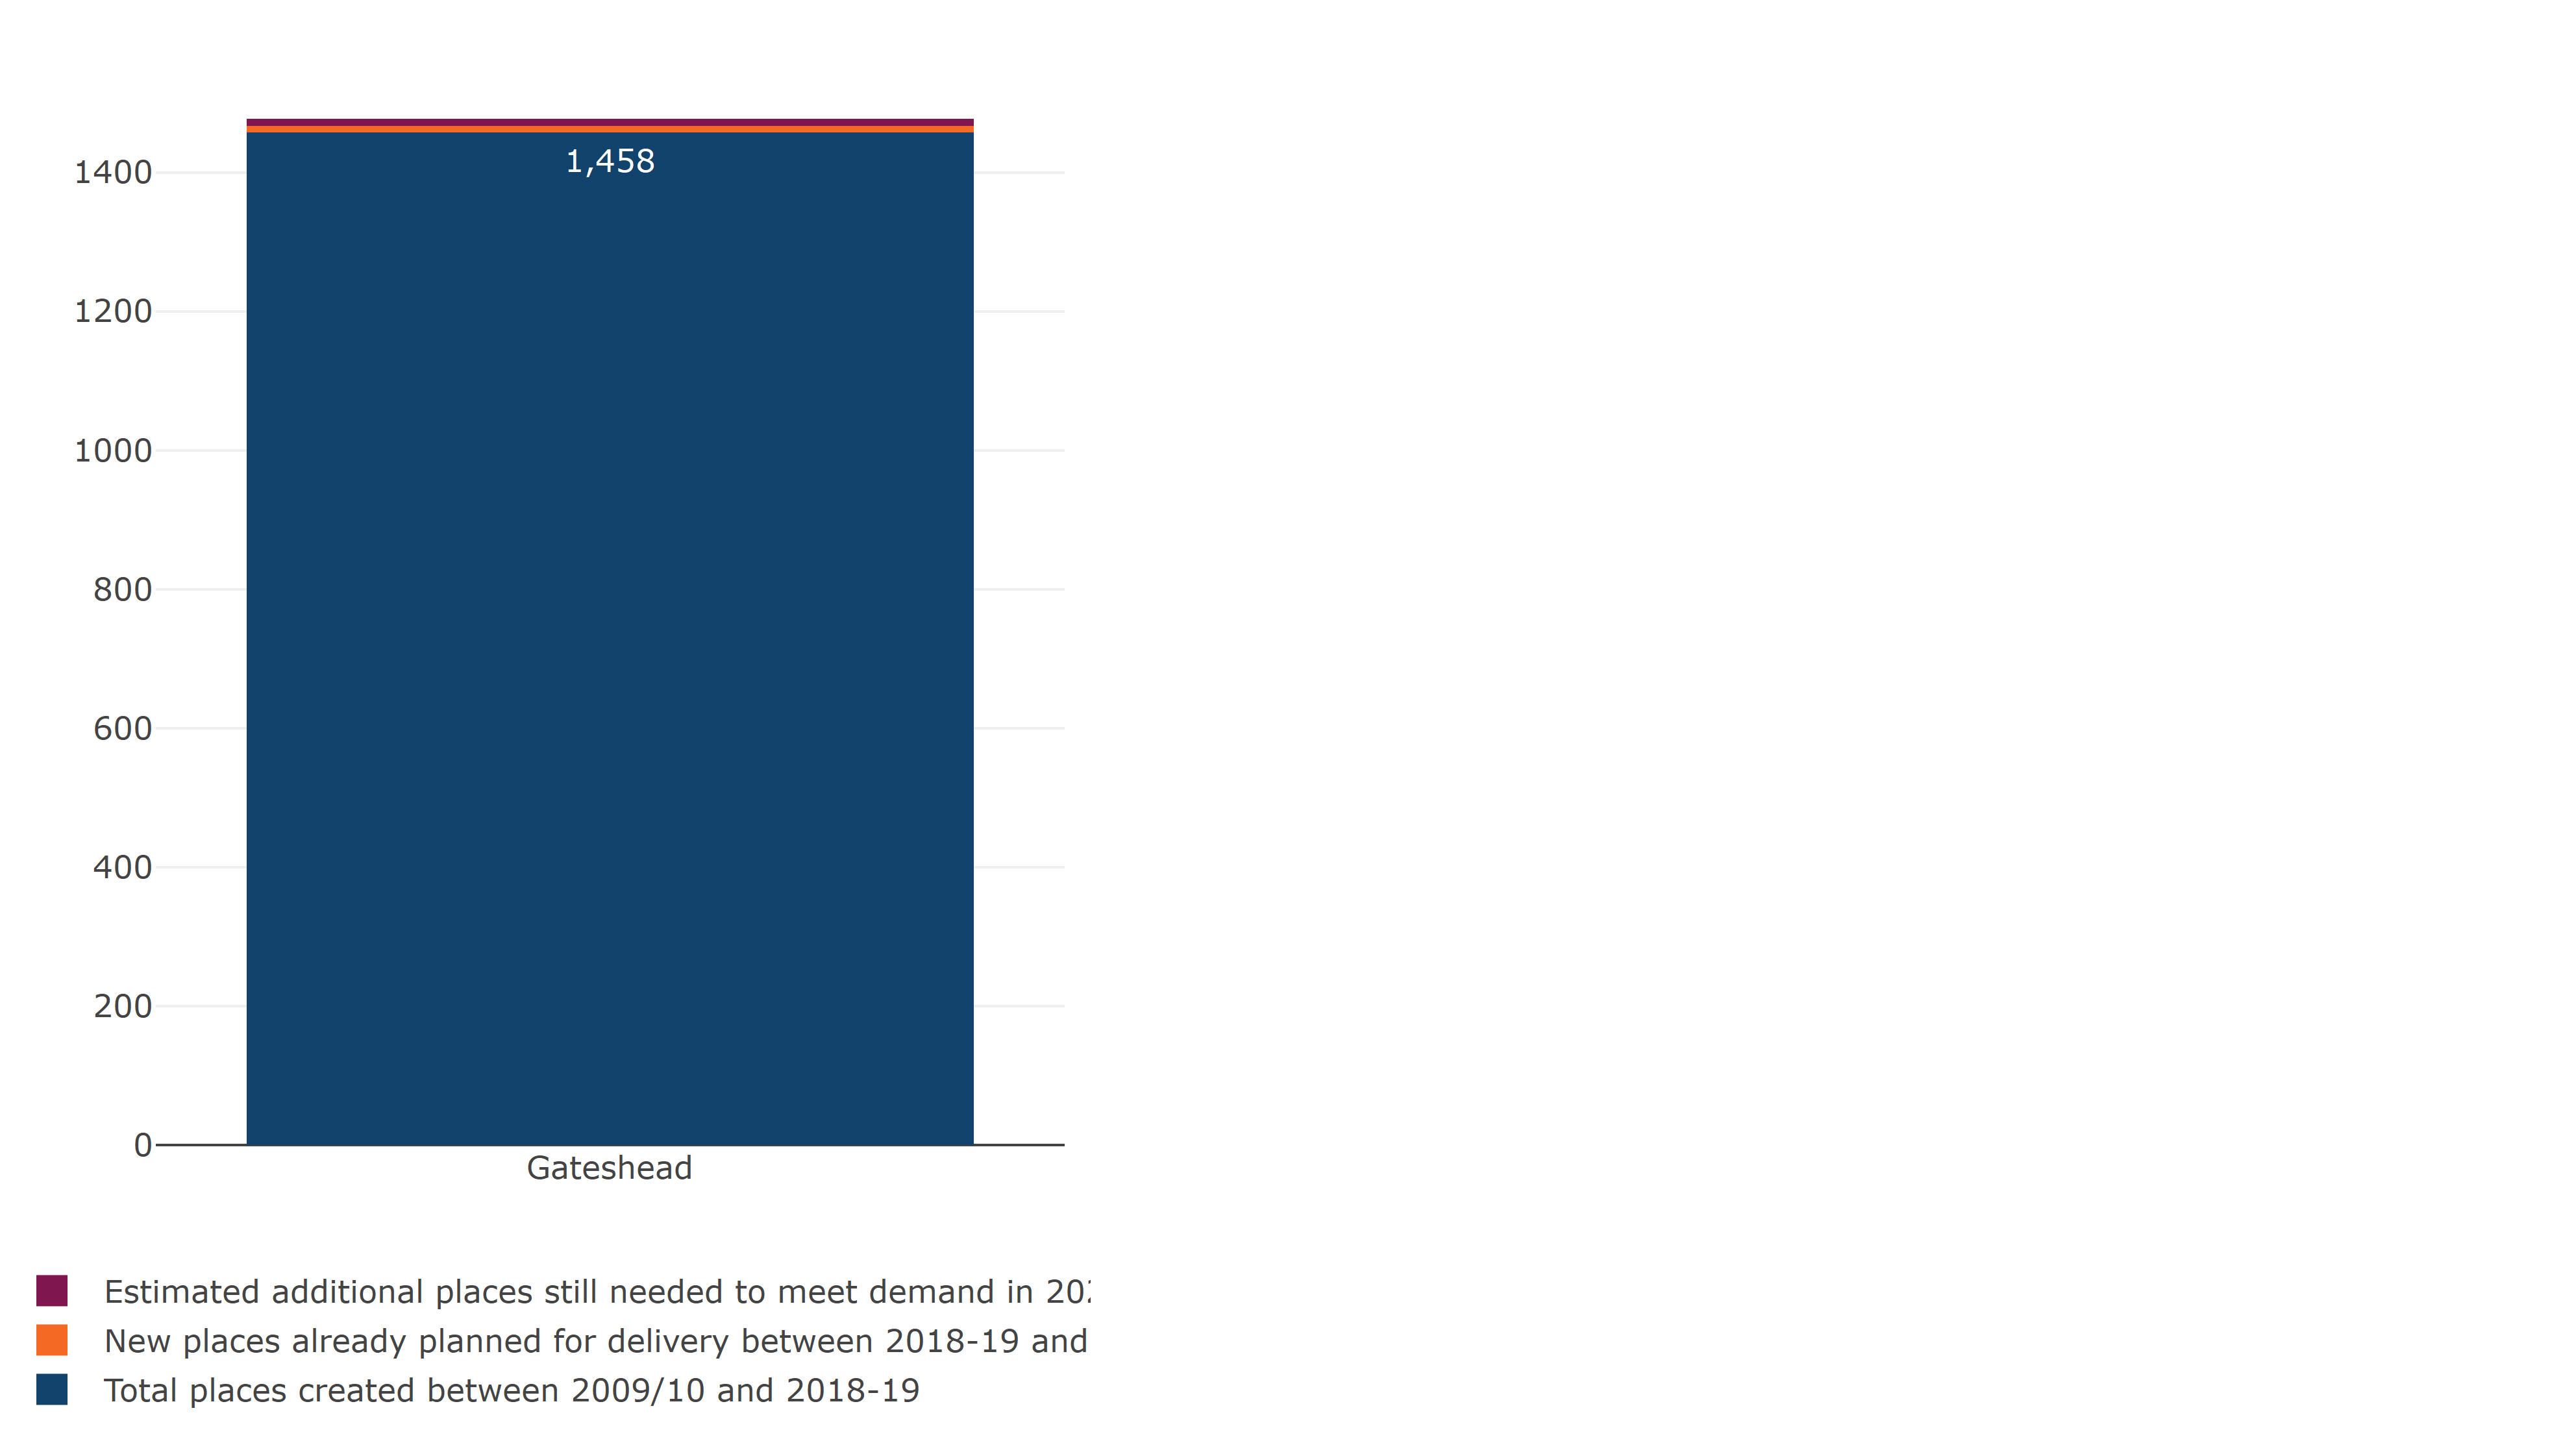
\includegraphics[width=1\linewidth]{Summary_scorecard_files/figure-latex/quantity_b-1}

\newpage

\hypertarget{preference}{%
\subsection{Preference}\label{preference}}

\hypertarget{proportion-of-applicants-who-received-an-offer-of-one-of-their-top-three-preference-schools-for-september-2019-entry}{%
\subsubsection{Proportion of applicants who received an offer of one of
their top three preference schools for September 2019
entry}\label{proportion-of-applicants-who-received-an-offer-of-one-of-their-top-three-preference-schools-for-september-2019-entry}}

\makebox[1.0\linewidth]{
\centering
\begin{tcolorbox}[colback=gssmidblue, 
 leftright skip=0.1cm,
 coltext=white, 
 halign=left, 
 fontupper={\Huge \bfseries},
 fontlower={\large \bfseries},
 sharp corners, 
 colframe=gssmidblue,
 width=0.49\linewidth,
 boxrule=0pt ,
 equal height group=prefbox
 ]
97.5\%
\tcblower
Percentage of applicants who recieved an offer of one of their top three preferred primary schools in England
\end{tcolorbox}
\begin{tcolorbox}[colback=gssmidblue, 
 leftright skip=0.1cm,
 coltext=white, 
 halign=left, 
 fontupper={\Huge \bfseries},
 fontlower={\large \bfseries},
 sharp corners, 
 colframe=gssmidblue,
 width=0.49\linewidth,
 boxrule=0pt,
 equal height group=prefbox
 ]
98.1\%
\tcblower
Percentage of applicants who recieved an offer of one of their top three preferred primary places in 2021-22 in Gateshead
\end{tcolorbox}
}

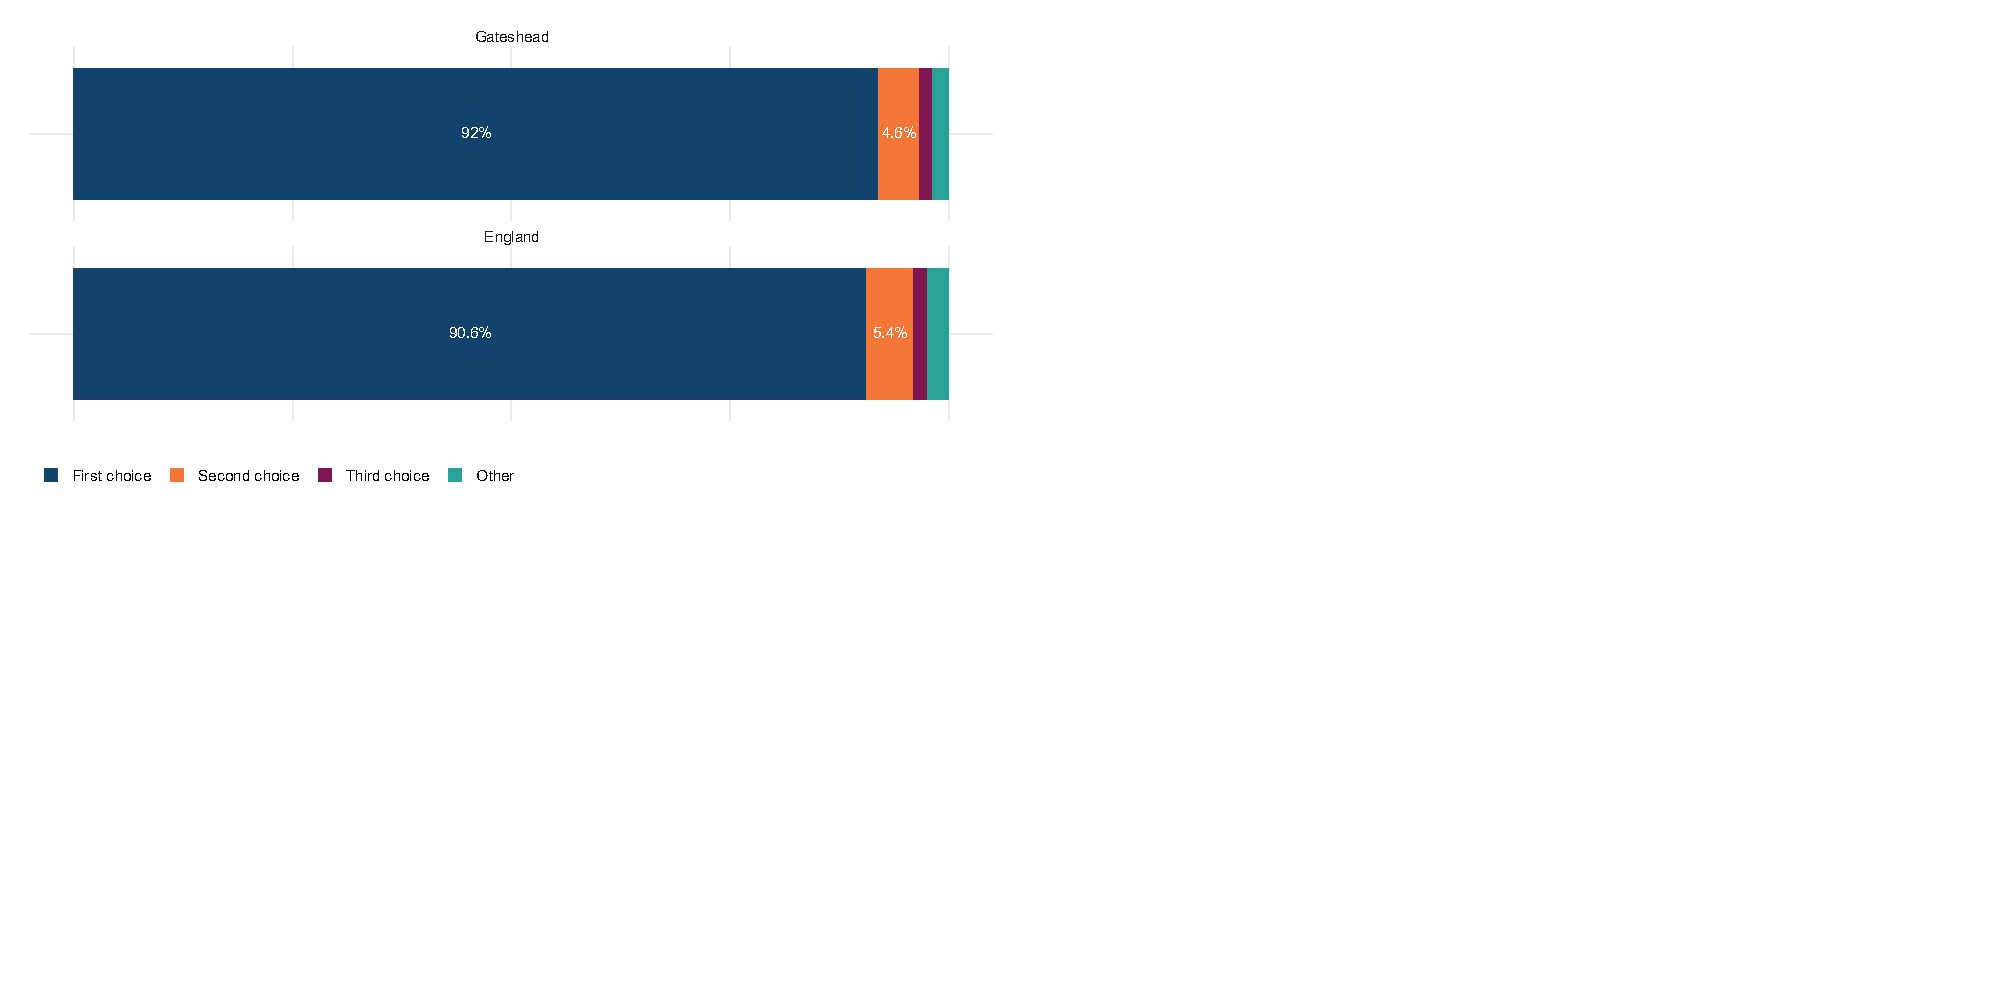
\includegraphics[width=1\linewidth]{Summary_scorecard_files/figure-latex/preference_barchart-1}

\newpage

\hypertarget{quality}{%
\subsection{Quality}\label{quality}}

\hypertarget{quality-of-places-created-between-2017-18-and-2018-19-based-on-ofsted}{%
\subsubsection{Quality of places created between 2017-18 and 2018-19,
based on
Ofsted:}\label{quality-of-places-created-between-2017-18-and-2018-19-based-on-ofsted}}

\makebox[1.0\linewidth]{
\centering
\begin{tcolorbox}[colback=gssmidblue, 
 leftright skip=0.1cm,
 coltext=white, 
 halign=left, 
 fontupper={\Huge \bfseries},
 fontlower={\large \bfseries},
 sharp corners, 
 colframe=gssmidblue,
 width=0.32\linewidth,
 boxrule=0pt,
 equal height group=qualbox
 ]
91\%
\tcblower
Percentage of new places created in good and outstanding  primary schools in England
\end{tcolorbox}
\begin{tcolorbox}[colback=gssmidblue, 
 leftright skip=0.1cm,
 coltext=white, 
 halign=left, 
 fontupper={\Huge \bfseries},
 fontlower={\large \bfseries},
 sharp corners, 
 colframe=gssmidblue,
 width=0.32\linewidth,
 boxrule=0pt,
 equal height group=qualbox 
 ]
64\%
\tcblower
Percentage of new places created in good and outstanding primary schools in Gateshead
\end{tcolorbox}
\begin{tcolorbox}[colback=gssmidblue, 
 leftright skip=0.1cm,
 coltext=white, 
 halign=left, 
 fontupper={\Huge \bfseries},
 fontlower={\large \bfseries},
 sharp corners, 
 colframe=gssmidblue,
 width=0.32\linewidth,
 boxrule=0pt,
 equal height group=qualbox
 ]
110
\tcblower
LA Rank out of 120 LAs that created new places between 2017-18 and 2018-19 (ranks can be tied)
\end{tcolorbox}
}

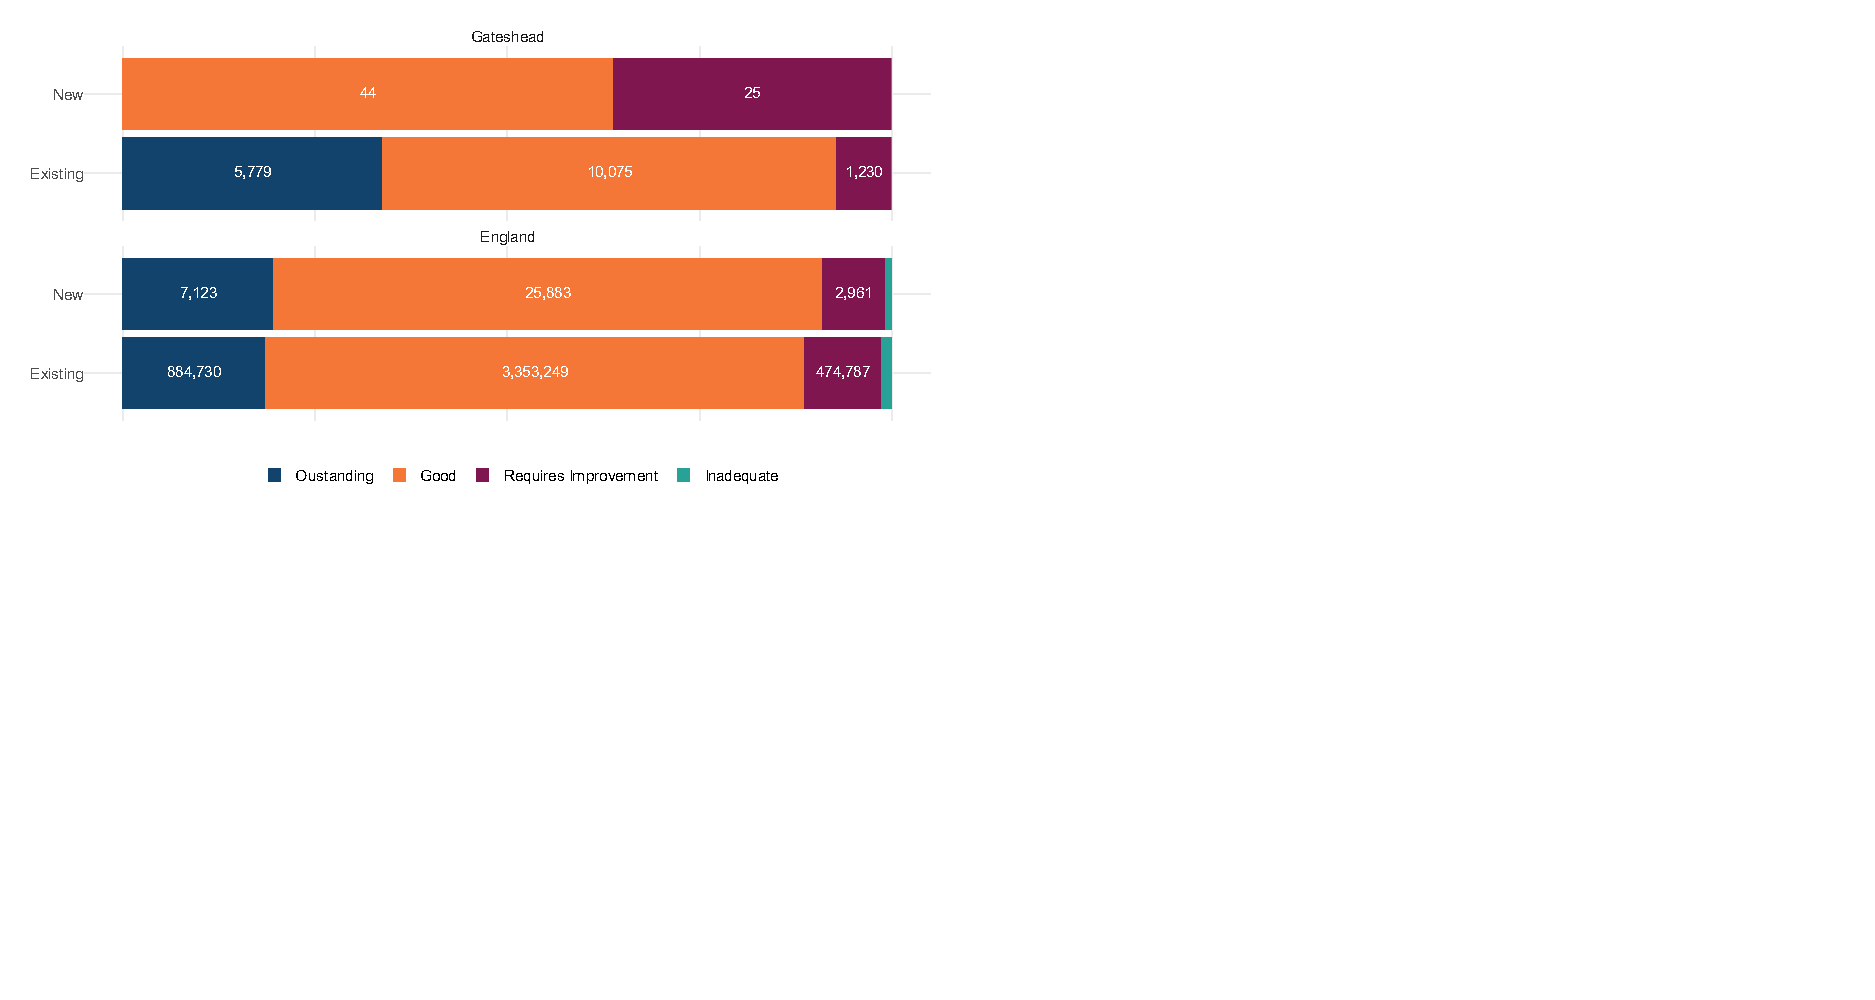
\includegraphics[width=0.92\linewidth]{Summary_scorecard_files/figure-latex/quality_chart-1}

New places with no rating = NA

\newpage

\hypertarget{cost}{%
\subsection{Cost}\label{cost}}

\# Cost
--------------------------------------------------------------------

\makebox[1.0\linewidth]{
\centering
\begin{tcolorbox}[colback=gssmidblue, 
 leftright skip=0.1cm,
 coltext=white, 
 halign=left, 
 fontupper={\Huge \bfseries},
 fontlower={\large \bfseries},
 sharp corners, 
 colframe=gssmidblue,
 width=0.32\\linewidth,
 boxrule=0pt,
 equal height group=costbox
 ]
91\%
\tcblower
Percentage of new places created in good and outstanding  primary schools in England
\end{tcolorbox}

\begin{tcolorbox}[colback=gssmidblue, 
 leftright skip=0.1cm,
 coltext=white, 
 halign=left, 
 fontupper={\Huge \bfseries},
 fontlower={\large \bfseries},
 sharp corners, 
 colframe=gssmidblue,
 width=0.32\\linewidth,
 boxrule=0pt,
 equal height group=costbox
 ]
91\%
\tcblower
Percentage of new places created in primary schools in England
\end{tcolorbox}

\begin{tcolorbox}[colback=gssmidblue, 
 leftright skip=0.1cm,
 coltext=white, 
 halign=left, 
 fontupper={\Huge \bfseries},
 fontlower={\large \bfseries},
 sharp corners, 
 colframe=gssmidblue,
 width=0.32\\linewidth,
 boxrule=0pt,
 equal height group=costbox
 ]
91\%
\tcblower
Percentage of new places created in good and outstanding  primary schools in England
\end{tcolorbox}
}

\begin{tabular}{l|l|l}
\hline
Type & England & North East\\
\hline
Permanent Expansion & £17,268 & £17,973\\
\hline
Temporary Expansion & £8,196 & -\\
\hline
New school & £20,508 & -\\
\hline
\end{tabular}

\begin{verbatim}
 paste0("The shaded area in each chart shows the forecasting accuracy for ", params$input_la_choice, ".
                 The starting point is 0: an accurate score.
                 A shared area to the right of 0 indicates an overestimate, a shared area to the left of 0 indicates an underestimate.")


 forecast_accuracy <- live_scorecard_data %>%
  filter(name == "For_1") %>%
  as.data.frame()

forecast_accuracy$value <- forecast_accuracy$value %>% roundFiveUp(., 3) * 100

forecast_range <- scorecards_data_pivot %>%
  filter(
    name == "For_1",
    Phase == params$input_phase_choice
  )


range_values <- forecast_range %>%
  summarise(
    quantile = scales::percent(c(0., 0.25, 0.5, 0.75, 1.0)),
    accuracy = 100. * quantile(value, c(0., 0.25, 0.5, 0.75, 1.0), na.rm = TRUE)
  ) %>%
  as.data.frame()

range_values$accuracy[5] <- (ceiling(range_values$accuracy[5]))
range_values$accuracy[1] <- (ceiling(abs(range_values$accuracy[1])) * range_values$accuracy[1] / abs(range_values$accuracy[1]))
 ggplot(
  forecast_accuracy,
  aes(name, value,
      fill = value,
      text = paste0(params$input_la_choice, ": ", value, "%")
  )
) +
  geom_bar(stat = "identity", width = 100) +
  scale_fill_gradientn(
    colors = divergent_gradient,
    space = "Lab",
    limits = c(-0.75 * abs(range_values$accuracy[5]), 1.08 * abs(range_values$accuracy[5])),
  ) +
  ylim(range_values$accuracy[1], range_values$accuracy[5]) +
  theme_bw() +
  theme(
    legend.position = "none", axis.text.y = element_blank(),
    axis.ticks.y = element_blank(),
    text = element_text(size = 12)
  ) +
  geom_hline(yintercept = 0, linetype = "dotted") +
  geom_hline(yintercept = range_values$accuracy[2], color="Grey", linetype = "dashed") +
 # geom_hline(yintercept = 100. * (forecast_range %>% filter(LA_name == "England"))$value) +
  geom_hline(yintercept = range_values$accuracy[4], color="Grey", linetype = "dashed") +
  geom_hline(yintercept = forecast_accuracy$value, size = 1.) +
  labs(x = "", y = "Accuracy (%)") +
  coord_flip()
ggplotly(p, tooltip = c("text")) %>%
  layout(font = font_choice) %>%
  config(displayModeBar = FALSE)
\end{verbatim}

\})

\newpage
\vspace*{\fill}
\color{dfeheadingblue}{\hrule}
\color{black}

\hypertarget{contact}{%
\subsection{Contact}\label{contact}}

\begin{quote}
Pupil place planning team

Publication:
\href{https://explore-education-statistics.service.gov.uk/find-statistics/local-authority-school-places-scorecards}{Explore
Education Statistics: Local authority school places scorecards}

Dashboard:
\href{https://department-for-education.shinyapps.io/la-school-places-scorecards}{LA
School Places Scorecards}

Email:
\href{mailto:SCAP.PPP@education.gov.uk}{\nolinkurl{SCAP.PPP@education.gov.uk}}

This document was produced using the
\href{https://github.com/dfe-analytical-services}{DfE Analytical
Services} Rmarkdown template, which is available on GitHub as part of
our
\href{https://github.com/dfe-analytical-services/shiny-template}{R-Shiny
data dashboard template}.
\end{quote}

\href{https://www.gov.uk/government/organisations/department-for-education}{
\includegraphics[width=0.50\linewidth]{"images/Department_for_Education_long.png"}}

\end{document}
